\chapter{Simulations}

\subsection{Numerical Solutions to Cell Problems}
Following the developments done before to obtain effective equations governing the macroscopic mechanical behavior of cortical bone, one of the main difficulties to solve corresponds to the so-called cell problems, which contains in this case the non-linear component associated to the homogenized coefficients.
Such a PDE problem is characterized by a unique vector valued solution $\mathbf{N}^{rs} \in \mathbf{H}^1_{\#} (\mathbf{Y})$ for each $r,s \in \{1,\dots, d\}$ satisfying the elliptic PDE system:
\begin{equation*}
    \left \{
    \begin{array}{cc}
        - \partial_{y_j} \big[C_{ijkl}(\mathbf{y}) \mathbf{e}_{kl,y} \big( \mathbf{N}^{rs}(\mathbf{y}) \big)  \big] = \partial_{y_j} \big( C_{ijrs} (\mathbf{y}) \big)& \text{ in } \mathbf{Y} \\
        \big[ C_{ijkl}(\mathbf{y}) \mathbf{e}_{kl,\mathbf{y}}\big( N^{rs}(\mathbf{y}) \big) \big]n_j = 0 &  \forall \mathbf{y} \in \partial Y
    \end{array}
    \right.
\end{equation*}
where we are adding the condition 
\begin{equation*}
    \int_{\partial Y} N^{rs}(\mathbf{y}) \, d\mathbf{y} = 0
\end{equation*}
to obtain uniqueness, since the right hand side of the problem has average $\mathbf{0}$.
The variational formulation is then giving by integration by parts, where for $\phi \in \mathbf{H}^1_{\#}(\mathbf{Y})$ we have
\begin{equation*}
    \int_{Y} C_{ijkl}(\mathbf{y}) \mathbf{e}_{kl,\mathbf{y}}(N^{rs}(\mathbf{y})) \partial_{y_j}\phi_i = - \int_{Y}C_{ijrs}(\mathbf{y}) \partial_{y_j} \phi_i + \int_{\partial Y}C_{ijrs}(\mathbf{y}) n_j \phi_i
\end{equation*}

Considering the standard biomechanical literature, the bone matrix is mainly made from hydroxyapatite, a material which can be modeled with a linear elasticity behavior and inclusion defining the mesoscale composed mainly of fluid with principal component being water or viscous behavior which in this first approximation we consider static elastic water-like material. Taking radial symmetry, the composed compaterial is modeled with transverse isotropy in each component $C^m_{ijkl}$, $C^w_{ijkl}$ matrix and water phases respectively.
It follows then the elastic tensors $C_{ijkl}$ defined in the cell $\mathbf{Y}$ by
\begin{equation*}
    C_{ijkl} (\mathbf{y}) := C^m_{ijkl} \mathbb{I}_{\{\mathbf{y} \in  \mathbf{Y}_{m}\}} + C^w_{ijkl} \mathbb{I}_{\{ \mathbf{y} \in \mathbf{Y}_{w}\}}
\end{equation*}
Such isotropic elastic behavior can be described explicitely using \textit{Voigt} notation as a $6\times 6$ matrix in the 3-dimensional case by:
\begin{equation*}
    C_{ij}(\mathbf{y}) = 
    \begin{bmatrix}
    C_{11}(\mathbf{y}) & C_{12}(\mathbf{y}) & C_{13}(\mathbf{y}) & 0 & 0 & 0 \\
    C_{12}(\mathbf{y}) & C_{11}(\mathbf{y}) & C_{23}(\mathbf{y}) & 0 & 0 & 0 \\
    C_{13}(\mathbf{y}) & C_{23}(\mathbf{y}) & C_{23}(\mathbf{y}) & 0 & 0 & 0 \\
    0 & 0 & 0 & C_{44}(\mathbf{y}) & 0 & 0 \\
    0 & 0 & 0 & 0 & C_{44}(\mathbf{y}) & 0 \\
    0 & 0 & 0 & 0 & 0 & C_{66}(\mathbf{y}) 
    \end{bmatrix}
\end{equation*}

which is given by the symmetries of the transverse isotropy of the material components. In particular, we have that $C_{55}(\mathbf{y}) = C_{44}(\mathbf{y})$ and $C_{11}(\mathbf{y}) = C_{22}(\mathbf{y})$.

We consider then simulations of the homogenized coefficients in function of the porosity level, i.e., setting the circular inclusion with radious $r(p)$ being $p \in (0,1)$ the set of admissible porosity levels, in the form 
\begin{equation*}
    p := \frac{\vert \mathbf{Y}_f \vert }{\vert \mathbf{Y}\vert} = \pi r(p)^2 \implies r(p) := \sqrt{\frac{p}{\pi}}
\end{equation*}

Explicitly, we consider an increasing array of possible porosity levels associated limited to the clinical interest intervals, i.e. we limit ourselves to the interval $[0, 0.3]$ of possible porosities. The numerical solution to the model is done using the UFL language implemented within the library FEniCS\footnote{The FEniCS project is an international initiative, started in 2013 with the objective to automate the solution of mathematical models based of Partial Differential Equations, for example of the type elliptic as the heat equation, hyperbolic as the wave equation, quasi-hyperbolic equations, etc., using the Finite Element theory and formalism to find such solution. More in general, its capable to find an approximate solution by means of a well-posed general variational formulation. \\
Defined as a set of interdependent base \texttt{C++} libraries such as \texttt{DOLFIN}, \texttt{FIAT}, \texttt{SFC} to just mention some, FEniCS implements an close-to-abstract coding and procedure to solve PDE problems on interface languages such as the native \texttt{C++} or via wrappers \texttt{Python}. Moreover, such base libraries rely on high-performance libraries for the algebra computations necessary in the FEM, such as \texttt{PETSc} which implements iterative solver of \textit{Krylov} type and a range of preconditioner to find an approximate solution $x \in \mathbb{R}^m$ of $Ax = b$ for $\mathcal{M}_{m \times m}(\mathbb{R})$, $b \in \mathbb{R}^m$ for $m \gg 1$.} to solve PDE in variational formulation.

In particular, it's used the \texttt{PETScKrylov} solver to solve the matrix system obtained after discretize the variational formulation by FEM, and over such solver we used the \texttt{GMRES} (Generalized Minimal Residual Method)\footnote{The \texttt{GMRES} method is an efficient algorithm to solve large linear systems. It uses an iterative method associated to the Theory of Krylov subspaces to approximate the solution of the system by reducing the high dimensional problem to a sequence of low dimensional, solved each one by least squares.
Explicitly, given $A \in \mathcal{M}_{m\times m} (\mathbb{R})$, $b \in \mathbb{R}^m$ for $m\gg 1$, the \texttt{GMRES} algorithm solves the problem $A x = b$ by solving the problems 
\begin{equation*}
    \underset{x \in \mathcal{K}_n}{\text{ min }} \Vert b - Ax \Vert_2   
\end{equation*} 
for increasing values of $n \in \mathbb{N}$, knowing $\mathcal{K}_n = \mathcal{K}_n(A,b)$ the Krylov space of order $n$ defined by
\begin{equation*}
 \mathcal{K}_n(A,b) = \text{span }\{ b, Ab, \dots, A^{n-1}b \} \subset \mathbb{R}^m   
\end{equation*}
At each iteration, its computed the residual by least squares, where under reasonable assumptions of symmetry of the matrix, the residual will be sufficiently small for $n \ll m$.} with preconditioner given by \textit{iLU} (incomplete LU factorization). Such consideration where done to obtain convergence with stable results.

The results are then compared with the approximation of the homogenized coefficients for cortical bone using the same input coefficient data of \cite{Parnell2008}.

\begin{figure}[!h]
	\centering
	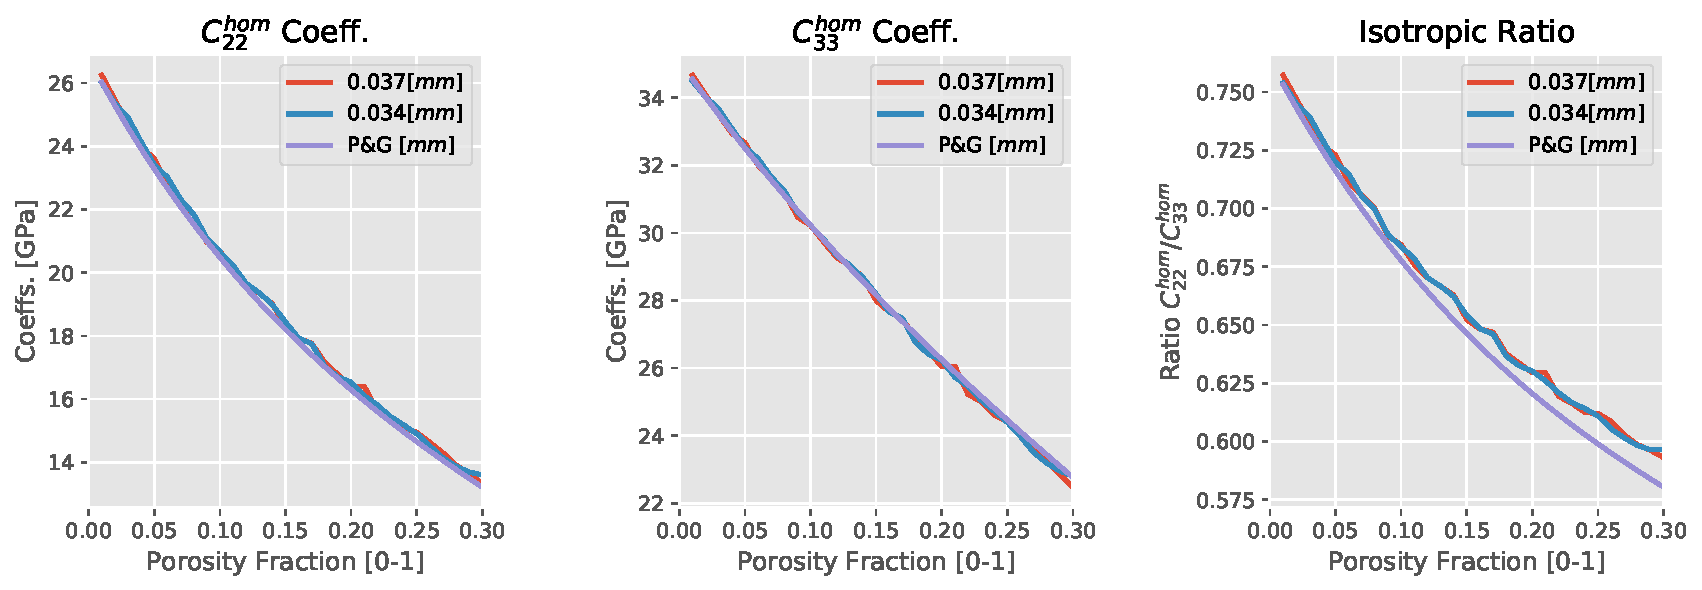
\includegraphics[scale=.5]{images/CellsProb/CellProb_MainHomCoeffsCircular.pdf}
	\caption{Main diagonal elastic homogenized coefficients in \textit{Voigt} notation. They describe an transverse isotropic behavior, spanned in the figure on the biomedical range of $(1,30) [\%]$ cortical porosity. The characteristic microstructure in this case is of unitary square.}
	\label{MainHomCoeffsSquare}
\end{figure}

\begin{figure}[!h]
	\centering
	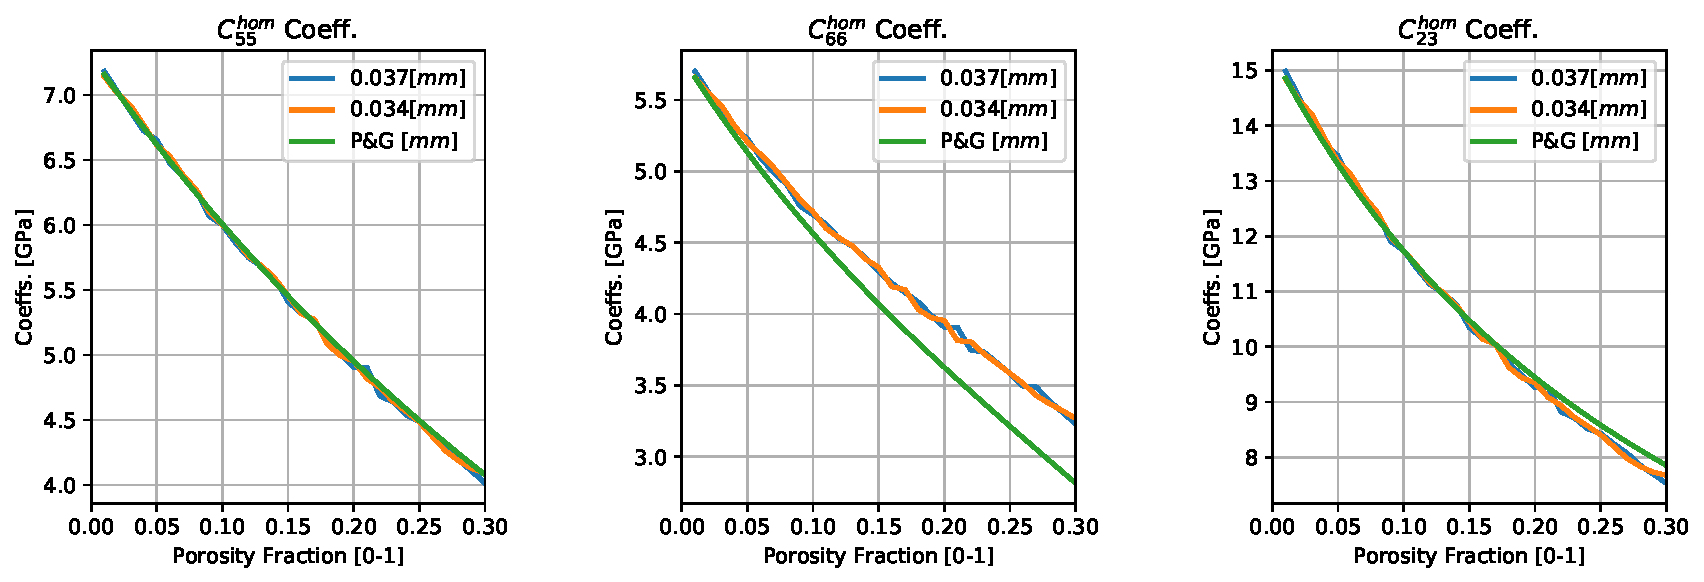
\includegraphics[scale=.5]{images/CellsProb/CellProb_OthersHomCoeffsCircular.pdf}
	\caption{Other diagonal elastic homogenized coefficients in \textit{Voigt} notation. They describe an transverse isotropic behavior, spanned in the figure on the biomedical range of $(1,30) [\%]$ cortical porosity with unitary square characteristic microstructure.}
	\label{OtherHomCoeffsSquare}
\end{figure}

\begin{center}
\begin{tabular}{ |p{2.5cm}||p{2cm}|p{2cm}|p{2cm}|p{2cm}| }
 \hline
 \multicolumn{5}{|c|}{Homogenized Coefficients} \\
 \hline
 Per. Error & $\phi = 5 \%$ & $\phi = 10 \%$ & $\phi = 15 \%$ & $\phi = 20 \%$ \\
 \hline
 $C^{hom}_{22}$ & 0.6 \% & 1.3 \% & 1.3 \% & 1.5 \% \\
 $C^{hom}_{33}$ & 0.1 \% & 0.1 \% & 0.1 \% & 0.1 \% \\
 $C^{hom}_{55}$ & 0.1 \% & 0.1 \% & 0.1 \% & 0.1 \% \\
 $C^{hom}_{66}$ & 1.4 \& & 3.3 \% & 6.3 \% & 9.0 \% \\
 $C^{hom}_{12}$ & 0.8 \% & 1.5 \% & 3.3 \% & 5.9 \% \\
 $C^{hom}_{23}$ & 0.4 \& & 0.1 \% & 0.3 \% & 1.0 \% \\
 \hline
\end{tabular}
\end{center}

\begin{rem}
It's important to note also the periodic microstructure idealization being used in \cite{Parnell2008} since it corresponds to an hexagonal structure defining the mesoscale, while the idealization proposed here is a square microstructure.
\end{rem}

Nevertheless, if we consider now a model using a microstructure as the one defined in \cite{Parnell2008}, i.e., as an hexagonal model with inclusions for the porosity level, the following results are obtained.

\begin{figure}[!h]
	\centering
	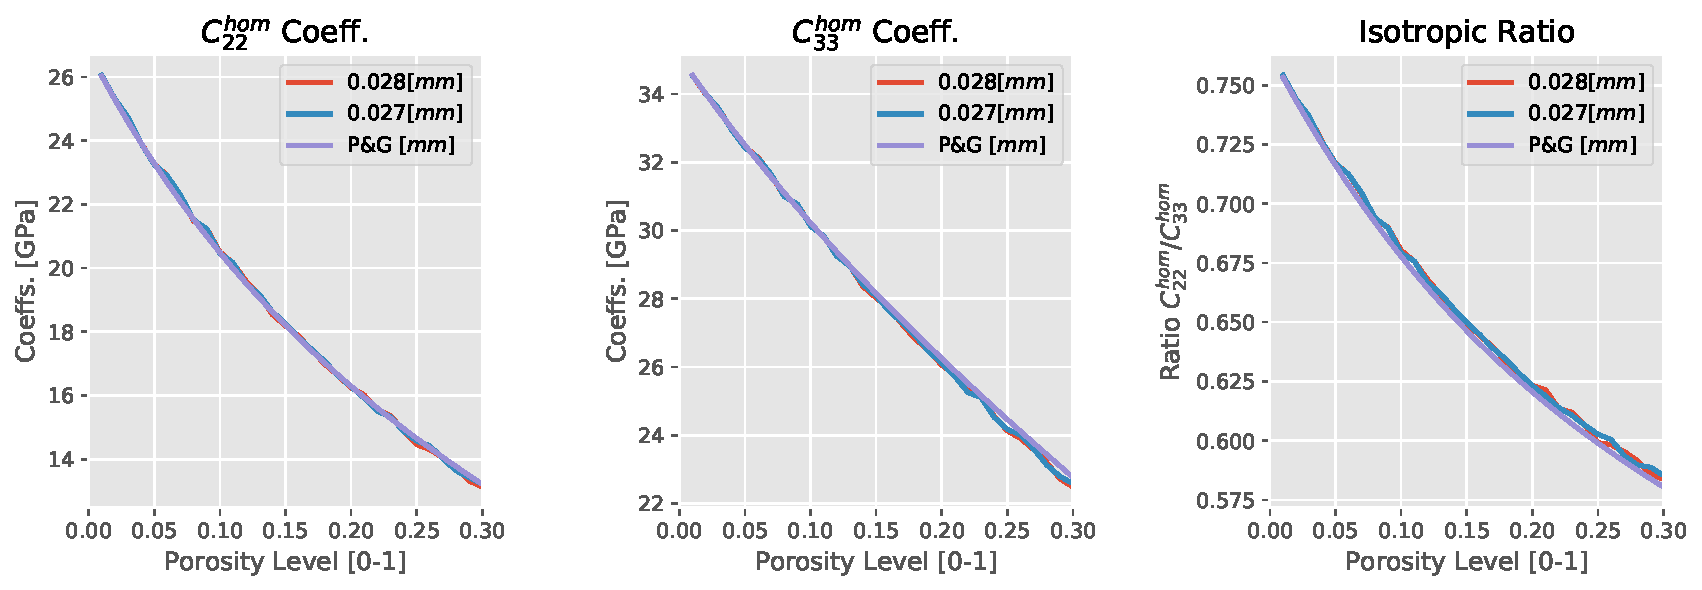
\includegraphics[scale=.5]{images/CellsProb/CellProb_MainHomCoeffsCircularHexa.pdf}
	\caption{Main diagonal elastic tensor coefficients in \textit{Voigt} notation. The figure shows the prediction values over the range $(1,30) [\%]$ of porosity with characteristic microstructure defined by an hexagonal 2-dimensional polygon.}
	\label{MainHomCoeffsHexagonal}
\end{figure}

\begin{figure}[!h]
	\centering
	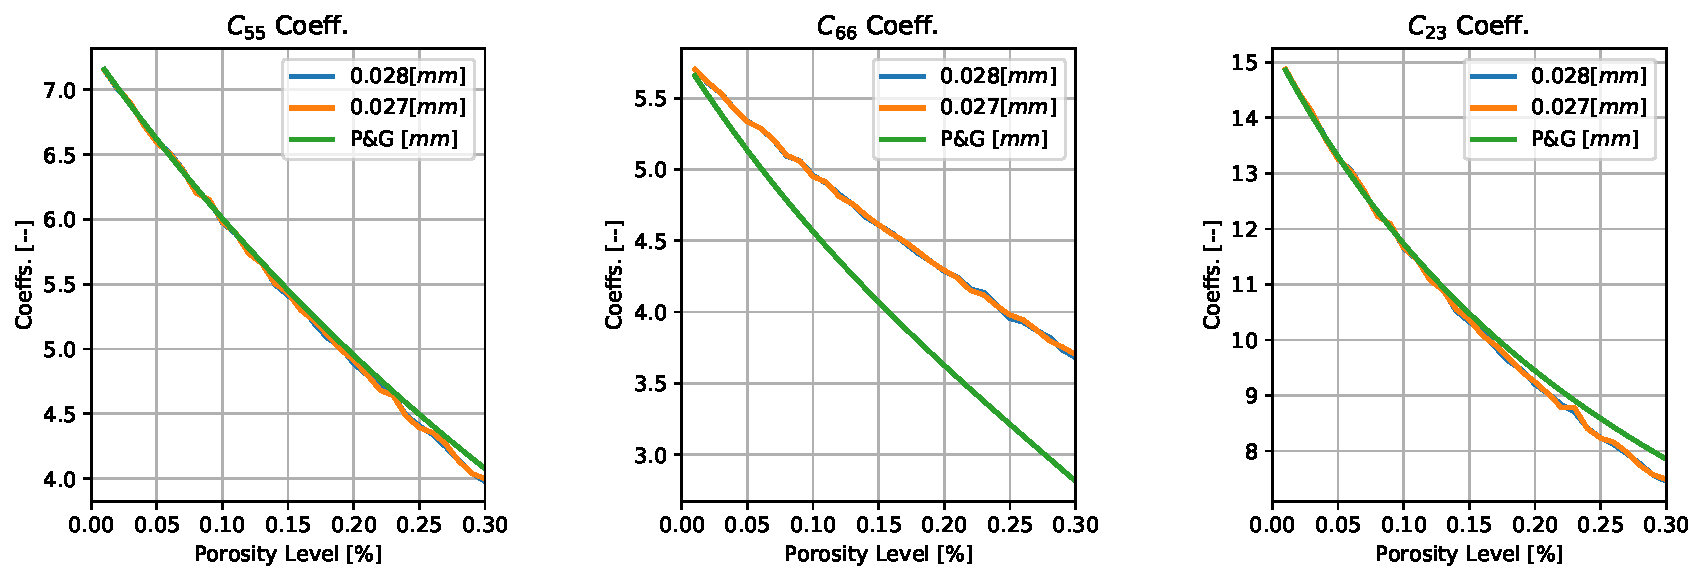
\includegraphics[scale=.5]{images/CellsProb/CellProb_OthersHomCoeffsCircularHexa.pdf}
	\caption{Shear type elastic homogenized coeffs. in \textit{Voigt} notation. The figure shows the behavior over the range $(1,30) [\%]$ porosity with characteristic microstructure described by a hexagonal 2-dimensional polygon.}
	\label{OtherHomCoeffsHexagonal}
\end{figure}

\subsection{Simulations of Wave Propagation}

The simulation setting associated to the experimental measurements is defined by a 2-dimensional rectangular array imitating the frontal plane associated to the cortical bone. The transducer excitation source is defined at the upper surface where the omit the interaction between the human skin and the bone structure itself. 
The experimental measurement procedure consist in the following steps:
\begin{itemize}
    \item Each source associated to the emission transductor is placed approximately at a distance of $0.5 \, [mm]$ from one another, being together a set of 8-12 different sources. 
    \item The detection is obtained by placing approximately from 24-72 sensors depending on the configuration used, where each one is placed at a distance approximately of $0.4 \, [mm]$ from one another.
\end{itemize}
Explicitly, the force acting is modeled in vertical direction associated to the horizontal plane of the skin pointing to the center of the cortical bone with a central time $t_0 > 0$ and oscillation speed $\tau_0 > 0$, i.e., described in the form:
\begin{equation}
    \mathbf{F}(\mathbf{x},t) = - e^{\frac{(t-t_0)^2}{2\sigma^2}} cos( 2 \pi t \tau_0 ) \mathbb{I}_{\mathbf{x} \in \Gamma_i} \hat{j} \quad \text{ on } \Gamma_N
\end{equation}
where $\{ \Gamma_i\}_{ i \in \{1,\dots, 8\}} \subset \Gamma_N$ denotes a disjoint subset of boundaries where the force is applied. 
Over such kind of configuration it can be proved theoretically the existence of the so-called \textit{Lamb}-waves that describe the particular propagation of guided waves associated to the elastic coefficients and density of the model being used.
In particular, the presence of a closed domain implies reflection with different directions related to the \textit{Neumann} or \textit{Dirichlet} respectively.

\subsubsection{Case of Multiple Sources}
Its simulated under the setting of 8 force sources positioned at equal distances of one to another. It defines then 8 different experiment thus wave-guided propagation with its recordings.
The figure \ref{FK-DiagramS8P12M10} describes the \textit{Lamb}-waves curves with the numerically simulated $(f,k)$-diagram. It shows the validation of the numerical model with respect to the theoretical prediction curves, observing clear correspondence between symmetrical and anti-symmetrical modes.

\begin{figure}[!h]
	\centering
	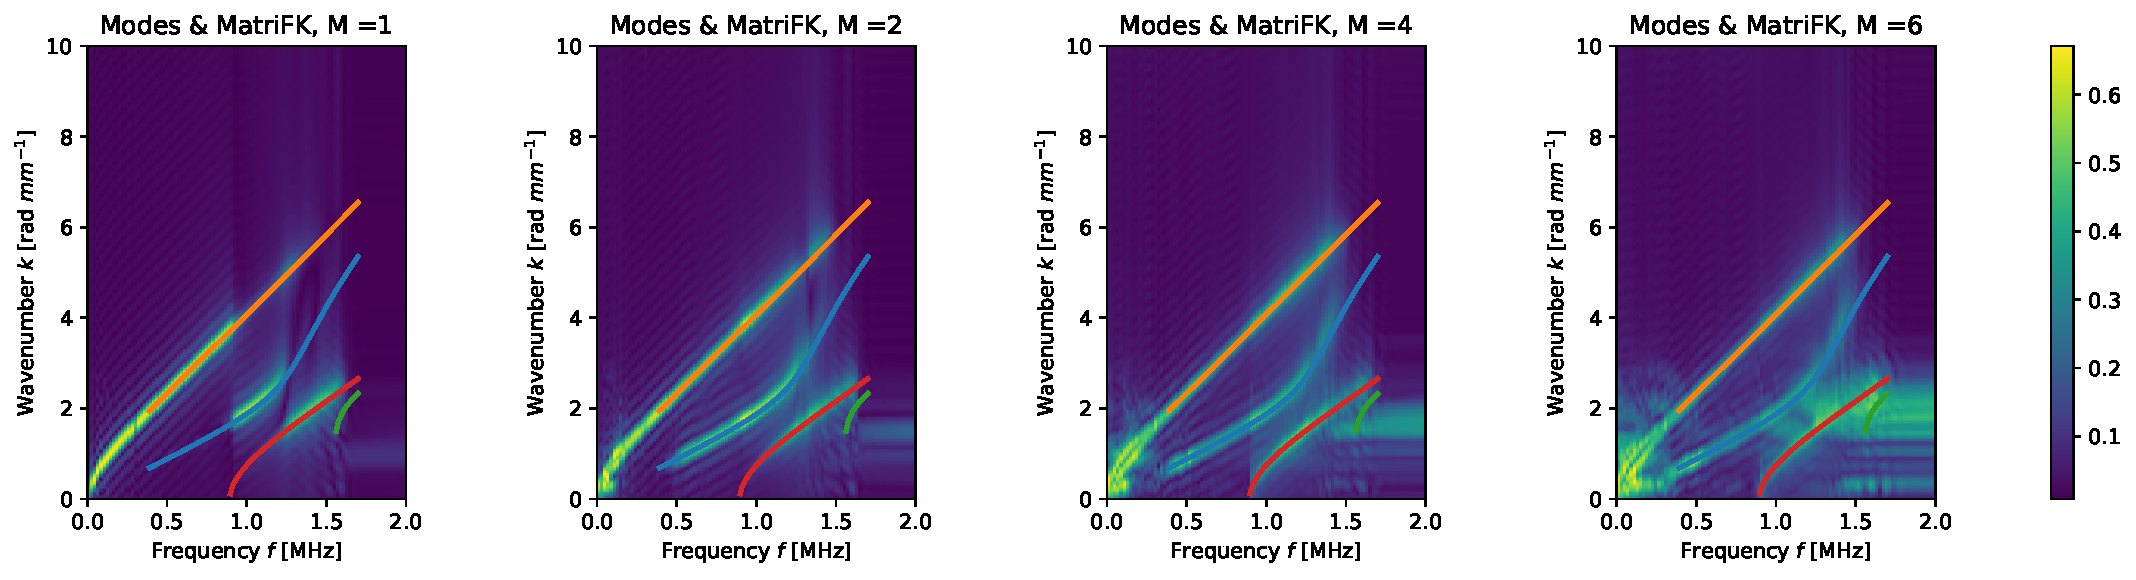
\includegraphics[width=\textwidth]{images/TimeMultSous/2DTimeS8P12ElasticFK10M780_y.pdf}
	\caption{Numerically Simulated $(f,k)$-diagram of 2D Transverse Elastodynamic Model: Setting of 8 sources with $12\%$ porosity and thickness of $1.0 [mm]$.}
	\label{FK-DiagramS8P12M10}
\end{figure}

Similarly \ref{SVD-S8P12M10} describes the modes in $[dB]$ from the singular value decomposition of the recording array. It shows the preponderance of the first three modes describing the wave-front.

\begin{figure}[!h]
	\centering
	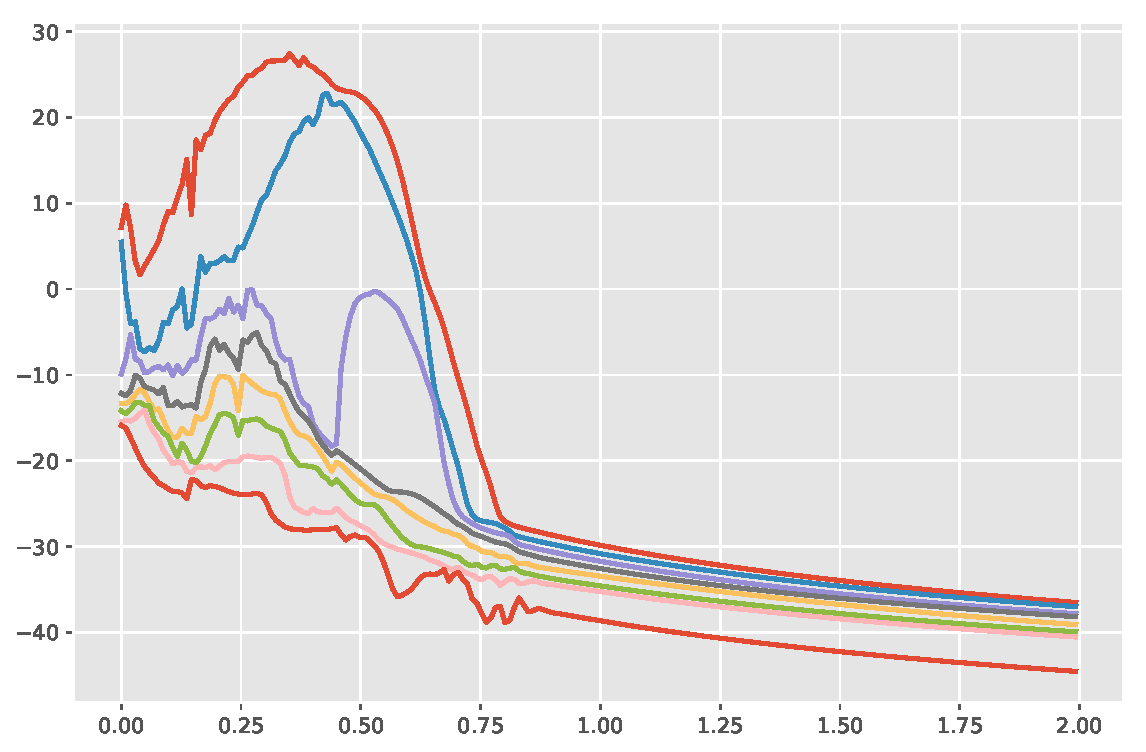
\includegraphics[scale=.5]{images/TimeMultSous/2DTimeS8P12Elastic10_SV.pdf}
	\caption{Singular values obtained by the SVD decomposition of the recorded signal from the simulation \ref{FK-DiagramS8P12M10}}
	\label{SVD-S8P12M10}
\end{figure}

The presence of several symmetric and antisymmetric modes expressed by the \textit{Lamb} waves is related experimentally with higher thickness values, since in this case the range of horizontal propagation is bigger.
Under such consideration, its shown on figure \ref{FK-DiagramS8P3M28} the wave-front simulations for a different pair $(Th., Po.)$, displaying a greater number of prediction curves.

\begin{figure}[!h]
	\centering
	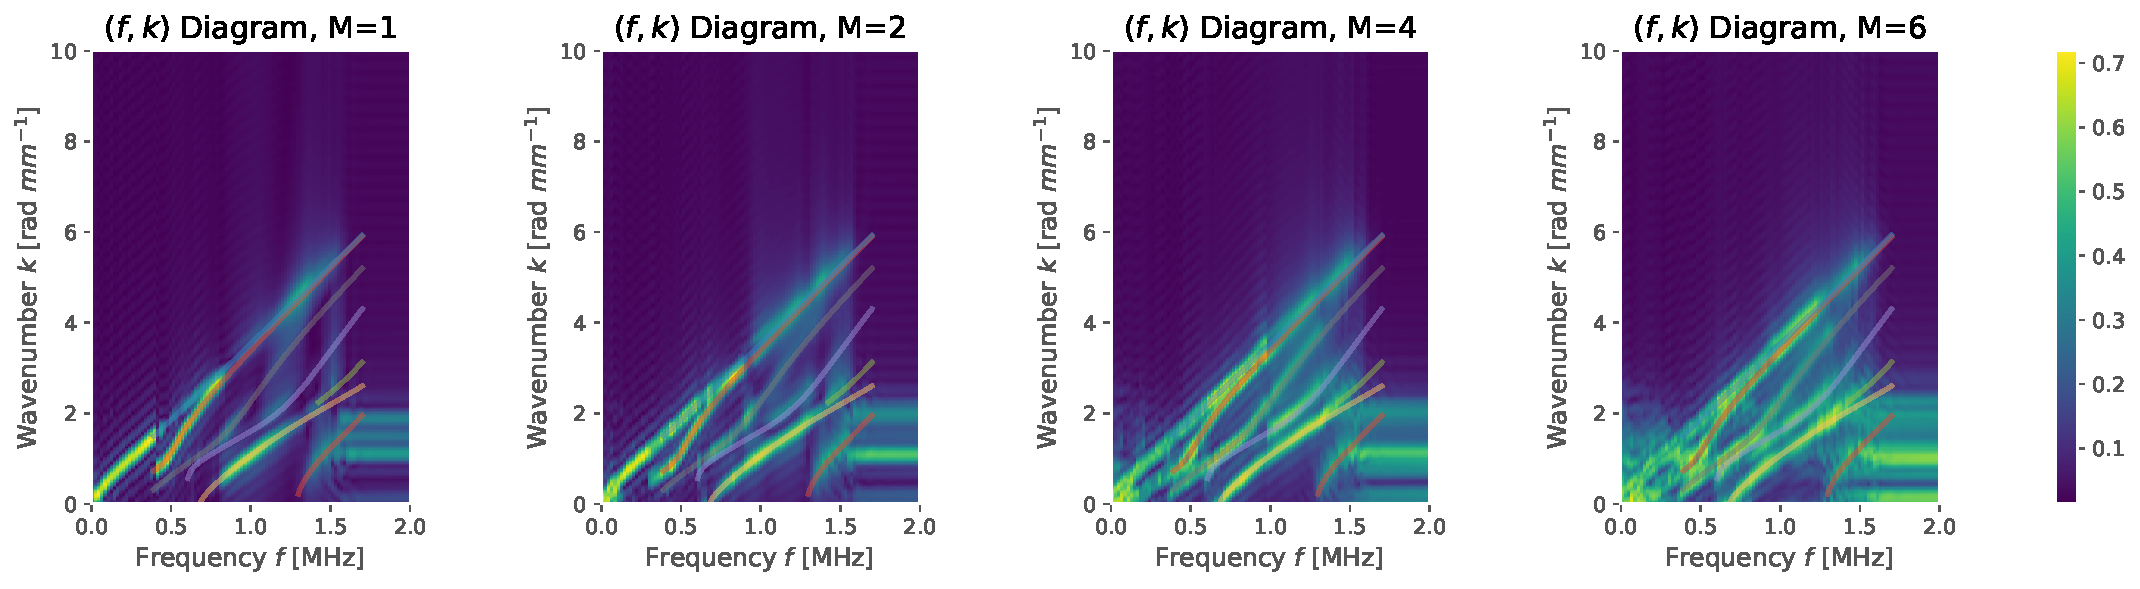
\includegraphics[width=\textwidth]{images/TimeMultSous/2DTimeS8P3ElasticFK28M780_y.pdf}
	\caption{Numerically Simulated $(f,k)$-diagram of 2D Transverse Elastodynamic Model: Setting of 8 sources with $3\%$ porosity and thickness of $2.8 [mm]$.}
	\label{FK-DiagramS8P3M28}
\end{figure}

Similarly, the corresponding modes in $[dB]$ from the singular value decomposition of the recording signal is shown on \ref{SVD-S8P3M28}, that compares naturally to the experimental reference literature.

\begin{figure}[!h]
	\centering
	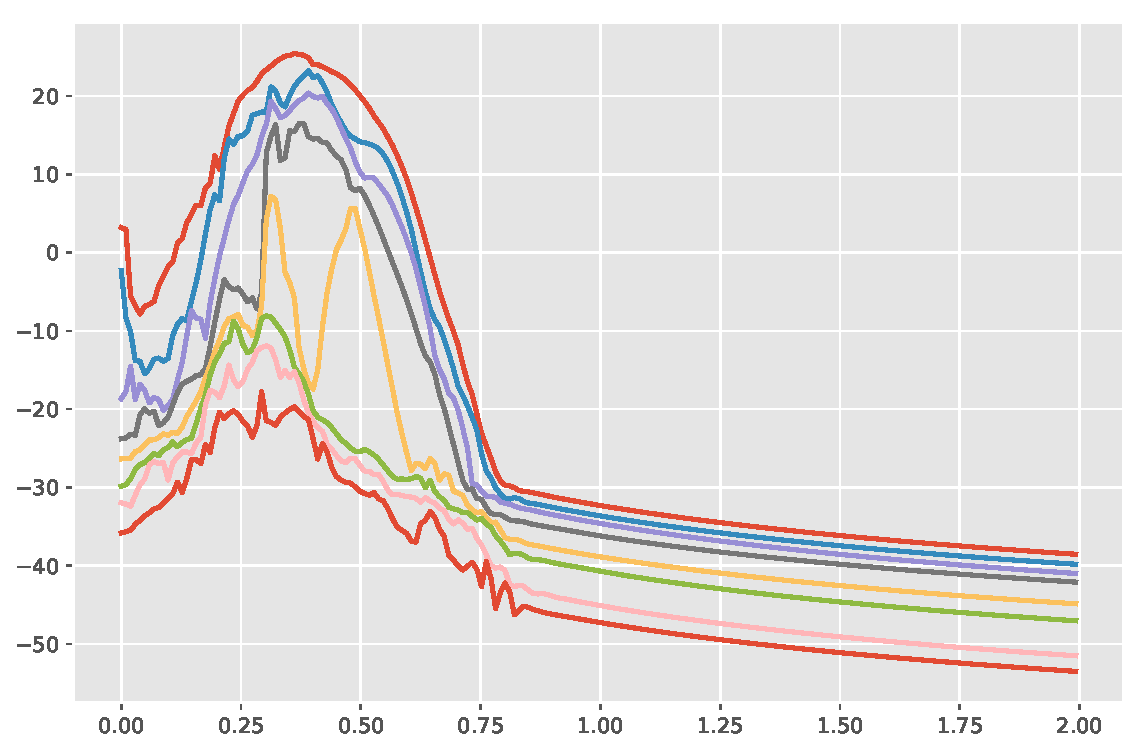
\includegraphics[scale=.5]{images/TimeMultSous/2DTimeS8P3Elastic28_SV.pdf}
	\caption{Singular values obtained by the SVD decomposition of the recorded signal from the simulation \ref{FK-DiagramS8P3M28}}
	\label{SVD-S8P3M28}
\end{figure}



\subsubsection{Case of a Single Source}
The above study of 8-source simulations to generate one sample of data introduces the problems of computational simulation under limited resources and time. 
To tackle such problem, its used the space invariance of the elastic wave since the recording to generate the output data array corresponds to just a space translation of the input signal for each one of the 8 propagation, thus such setting can be exchanged for one source with a higher number of sensors lowering the time-cost of the full simulation to 1/8 of the initial time.

Its shown then on figure \ref{FK-DiagramS1P6M33} the $(f,k)$-diagram associated to the 1-source simulations setting. It presents natural reflections related to the rectangular 2-dimensional domain used with mixed boundary conditions.
\begin{figure}[!h]
	\centering
	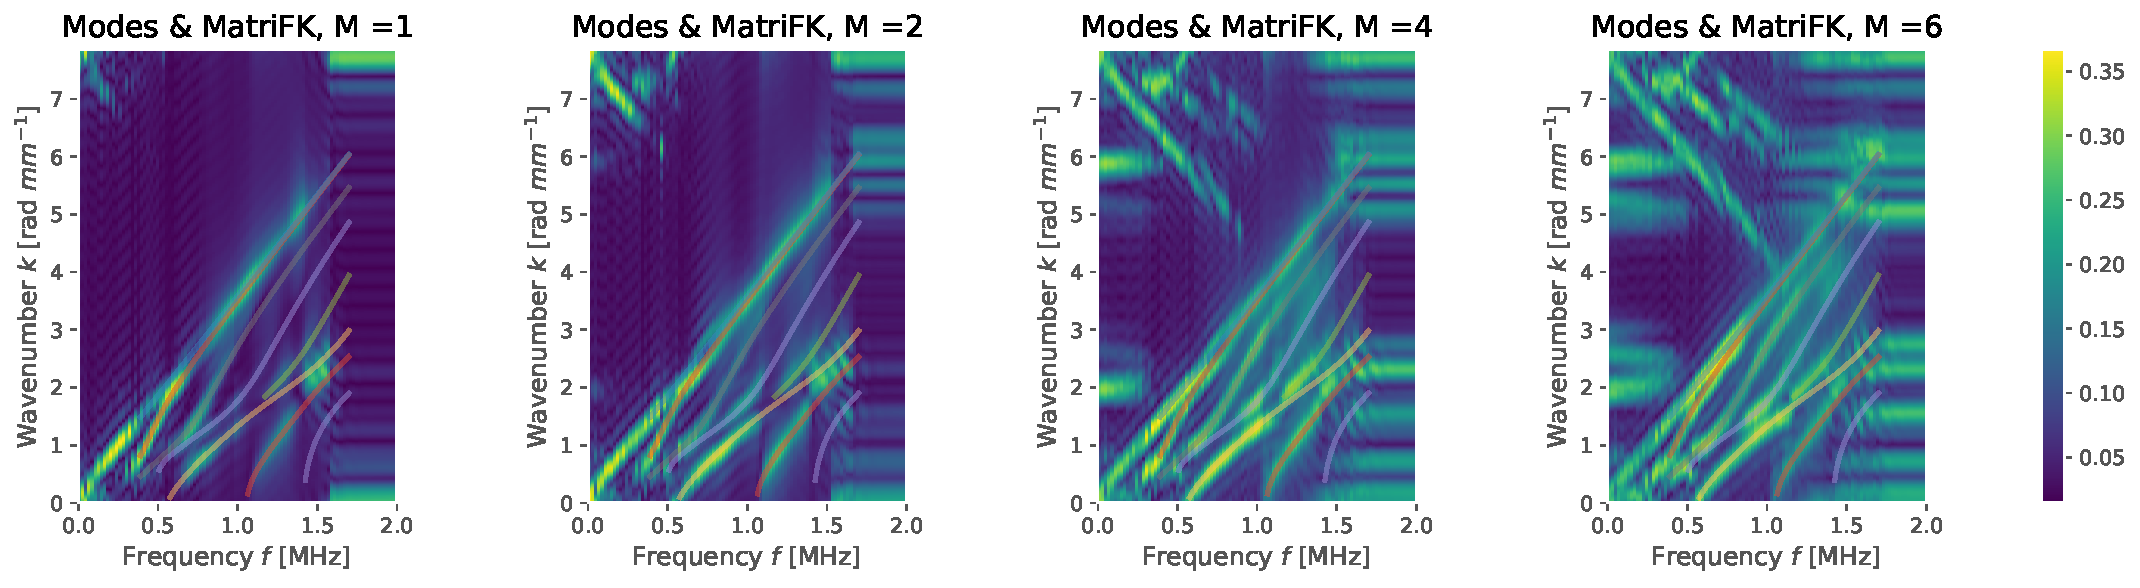
\includegraphics[width=\textwidth]{images/TimeSingSous/2DTime_P6ElasticFK33M1460_y.pdf}
	\caption{Numerically Simulated $(f,k)$-diagram of 2D Transverse Elastodynamic Model: Setting of 1 source with $6\%$ porosity and thickness of $3.3 [mm]$.}
	\label{FK-DiagramS1P6M33}
\end{figure}

Its shown moreover on figure \ref{SVD-S1P6M33} the main modes $[dB]$ associated to the recorded signal.
\begin{figure}[!h]
	\centering
	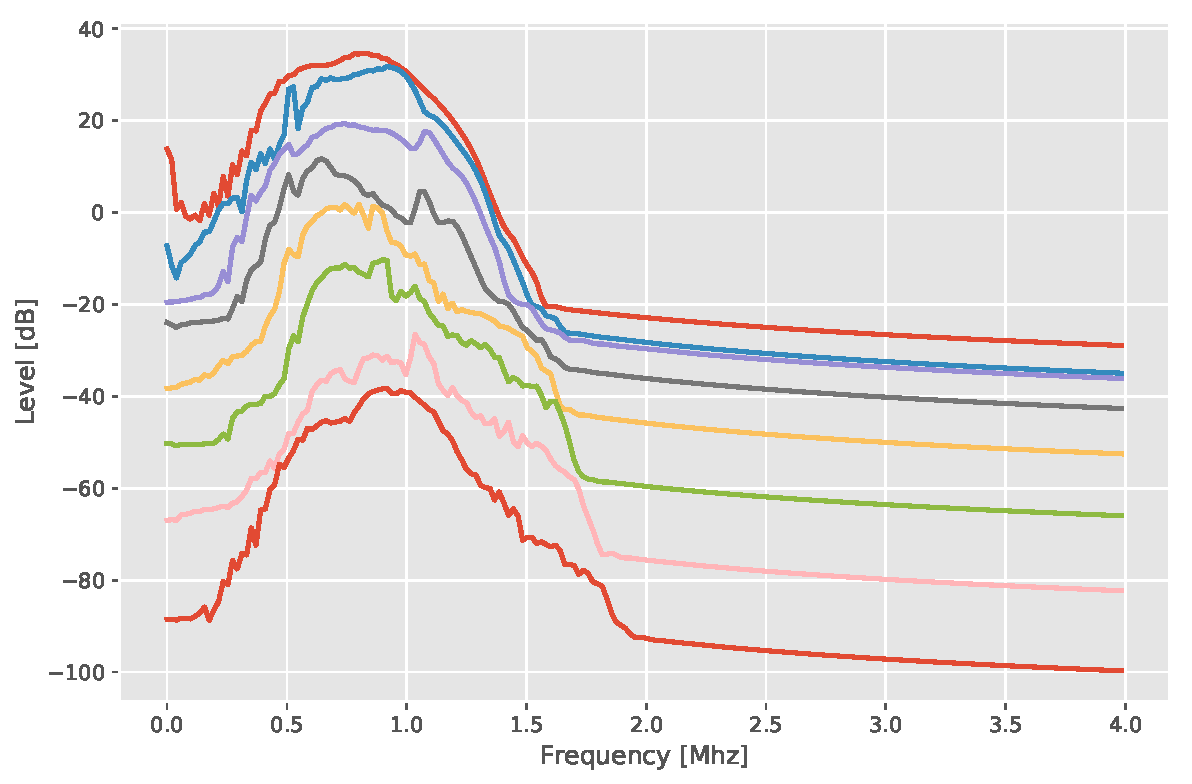
\includegraphics[scale=.5]{images/TimeSingSous/2DTime_P6Elastic33_SV.pdf}
	\caption{Singular values obtained by the SVD decomposition of the recorded signal from the simulation \ref{FK-DiagramS1P6M33}}
	\label{SVD-S1P6M33}
\end{figure}

The reflections shown in the image above produced from the simulations corresponds to an aliasing effect in the input signal $S(f_n, e_m, \mathbf{x}_p)_{(m,p) \in [N^E]\times [N^R]}$ after applying FFT over the space $[N^E] \times [N^R]$. Such aliasing express the folding of the $k$-variable \footnote{Associated to the wavenumber} by the conjugation property on \texttt{FFT}, i.e., 
\begin{equation*}
    \overline{\texttt{FFT}(S(f_n, \cdot, e_m))(k)} := \sum_{m=0}^M S(f_n, \mathbf{x}_p, e_m) \overline{e^{-2 \pi i \frac{p k}{M}}} = \texttt{FFT}(S(f_n, \cdot, e_m))(-k)
\end{equation*}
in such a way that the norm associated is the same. Moreover since we consider a finite wavenumber interval denoted $[0, k_{max}]$, such a reflected wavenumber is given by $k_{max}-k$ as observed in the figure.

Given such a symmetry, its considered the application of the analytic projector defined for a given signal $s$ regular enough by:
\begin{equation*}
    \mathcal{P}(s) := (I + \mathbf{i}\mathcal{H})(s)
\end{equation*}
being $\mathcal{H}$ the Hilbert transform. Such a projector defines the analytic signal of $s$ by constructing its real and imaginary parts.

Since the behavior observed in the $(f,k)$-diagrams are of symmetry, a natural idea is to use the \textit{Hilbert} transform on the input signal, obtaining a analytic signal which maintains the structure of the \textit{Lamb} modes and moreover recreates experimentally obtained results \textit{in-vivo} and \textit{ex-vivo}.
Applying then such a projection filter we obtain the results qualitatively and quantitatively similar with respect to the real experimental data.

\begin{figure}[!h]
	\centering
	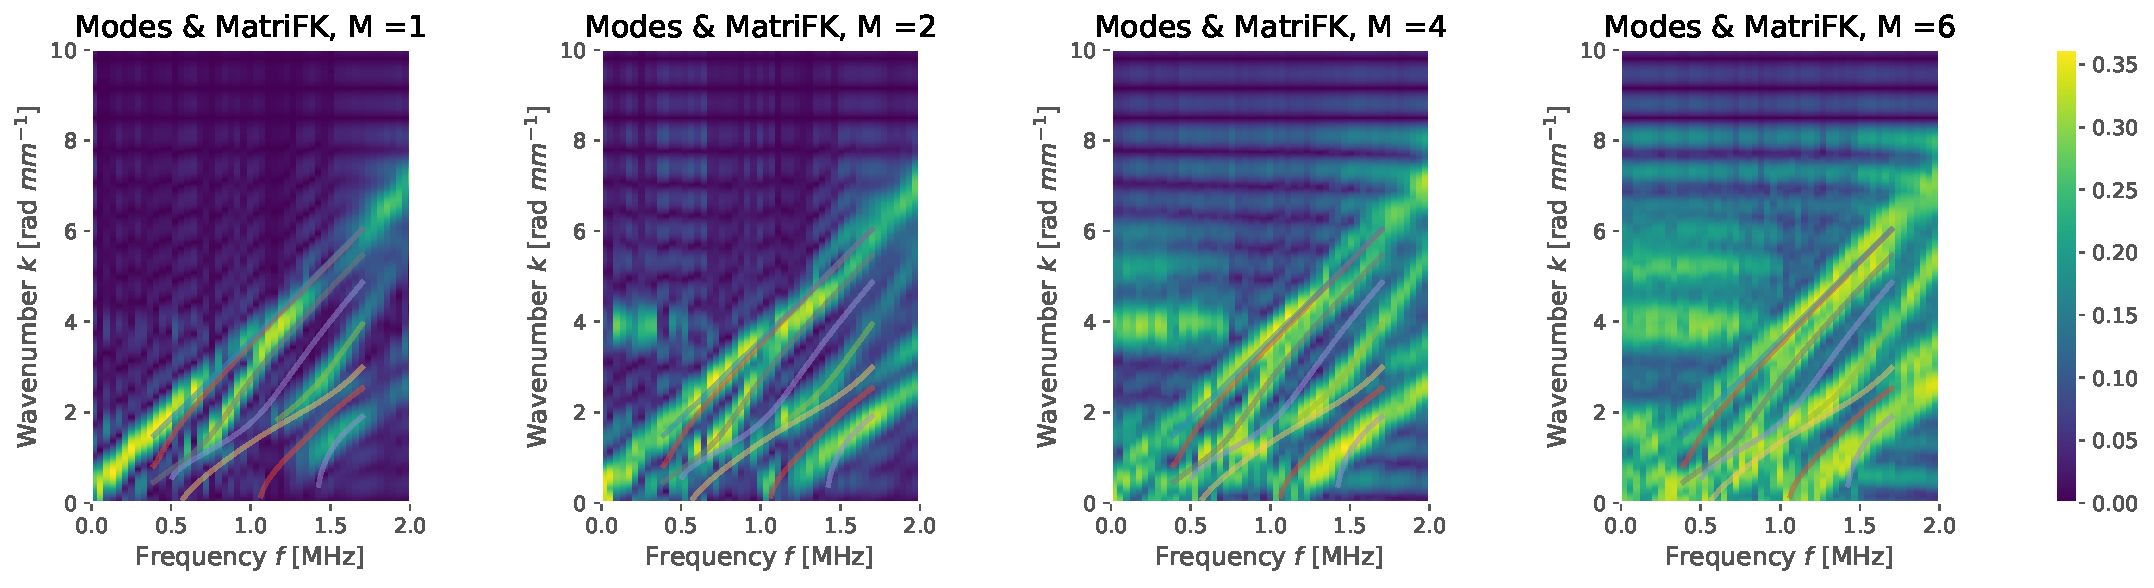
\includegraphics[width=\textwidth]{images/TimeSingSous/2DTimeHilb_P6ElasticFK33M1460_y.pdf}
	\caption{Numerically Simulated $(f,k)$-diagram of 2D Elastodynamic Model: Setting of 1 source with $6\%$ porosity and thickness of $3.3 [mm]$ appplying Hilbert transform to delete reflexions.}
	\label{FK-Hil-DiagramS1P6M33}
\end{figure} 

\begin{figure}[!h]  
	\centering
	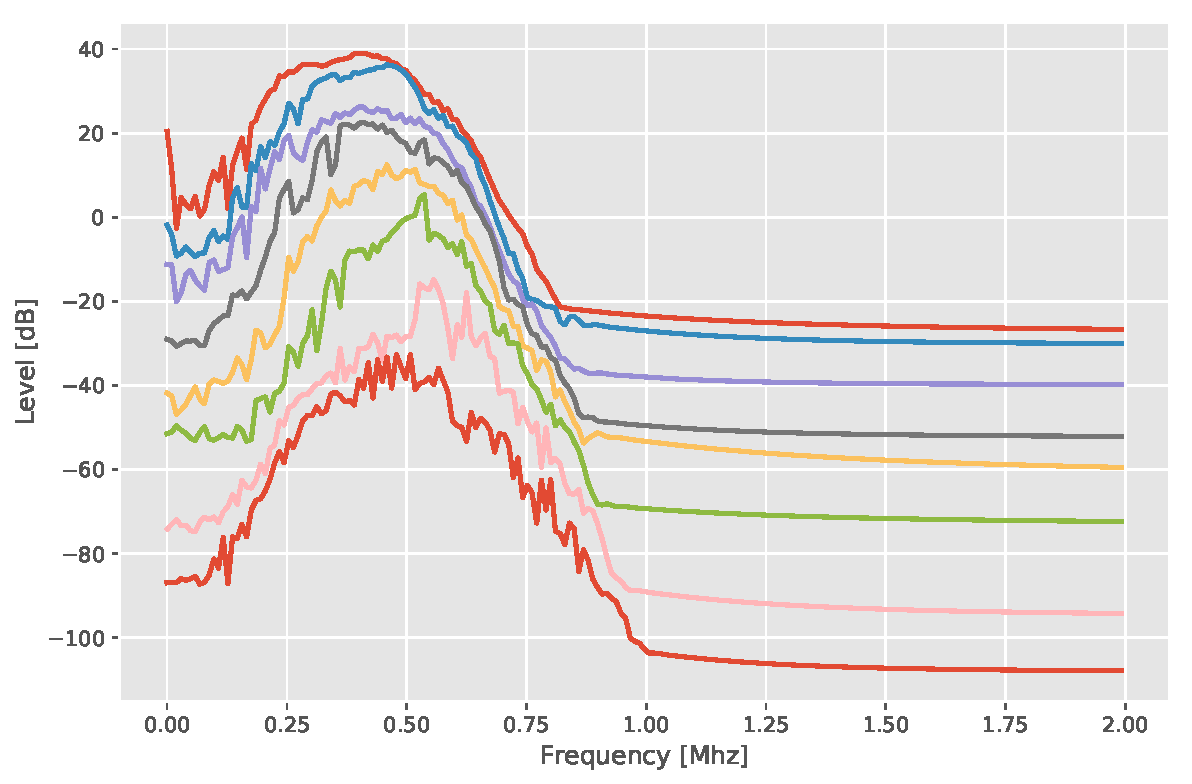
\includegraphics[scale=.5]{images/TimeSingSous/2DTimeHilb_P6Elastic33_SV.pdf}
	\caption{Singular values obtained by the SVD decomposition of the recorded signal from the simulation \ref{FK-Hil-DiagramS1P6M33}}
	\label{SVD-Hil-S1P7M33}
\end{figure}

\subsection{Case on Frequency Domain}

The time-domain simulation given results which represent qualitatively the model with enough fidelity, nevertheless such simulation requires a relatively small time step in such a way that the full simulation take considerable time. Thus, it is necessary to consider a model which reduces the computational cost.
To this end, taking into account that the signal processing involves the application of \texttt{FFT} over the sensors data, a straightforward method is to consider the simulations now in the time-domain over the arrays of frequencies that are of interest.

\subsubsection{Solutions without Attenuation}
In this case, using the schemes proposed in the section before showed results in which Lamb-Waves and also $dB$ figures where affected by distortions FIGURE BELOW. Such kind of behavior repeated over different pairs of porosity level and thickness associated to the simulations, in such a way that was necessary to study the spectrum of the elastic operator.

\begin{figure}[!h]
	\centering
	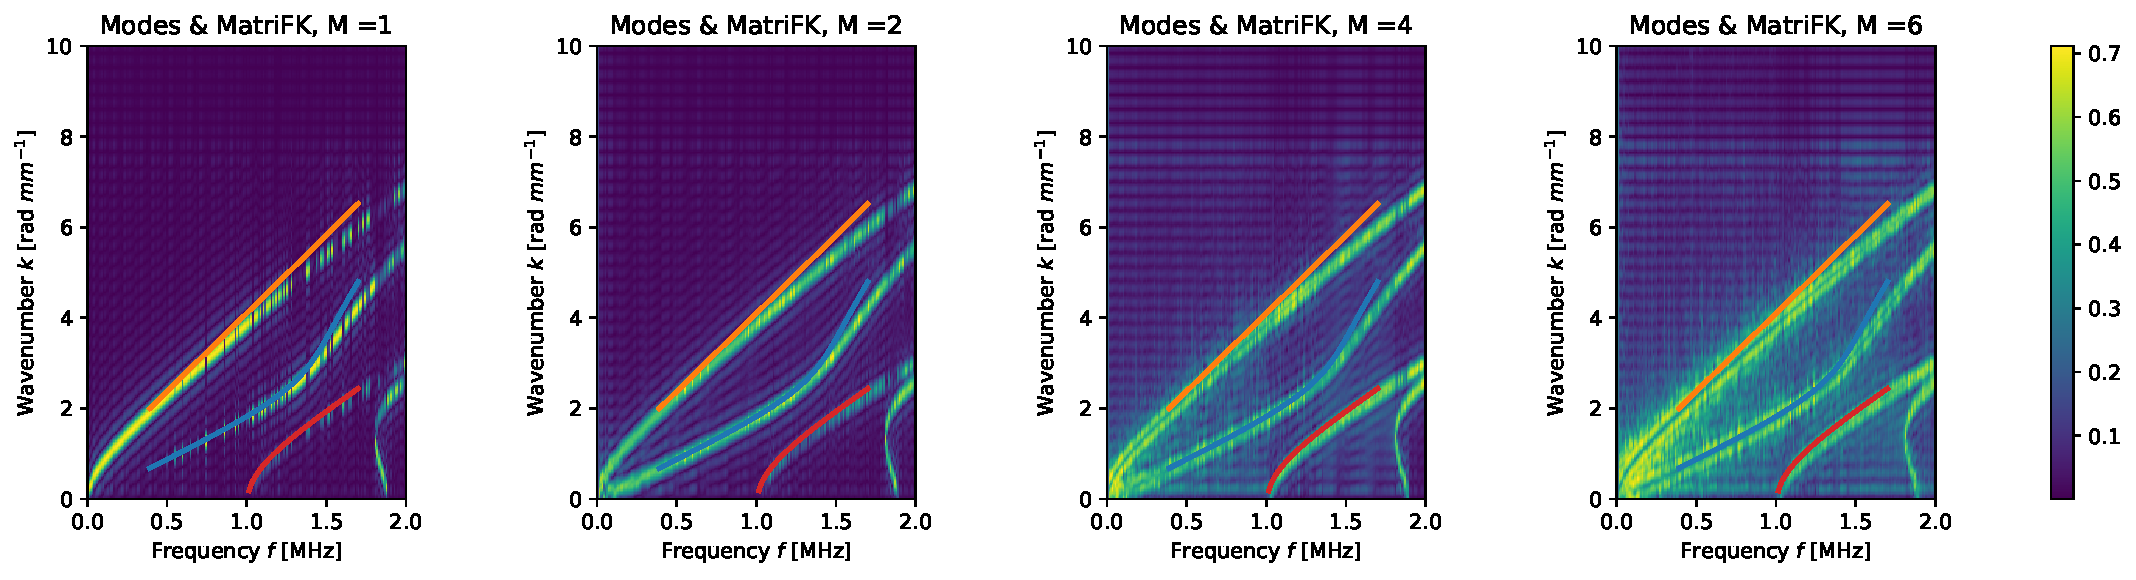
\includegraphics[width=\textwidth]{images/FreqRes/2DFreqS8P10ElasticFK09M300_y.pdf}
	\caption{Numerically Simulated $(f,k)$-diagram of 2D Elastic Model on Frequency Domain: Setting of 8 sources with $10\%$ porosity and thickness of $0.9 [mm]$}
	\label{FK-Freq-DiagramS8P10M09}
\end{figure} 

\begin{figure}[!h]
	\centering
	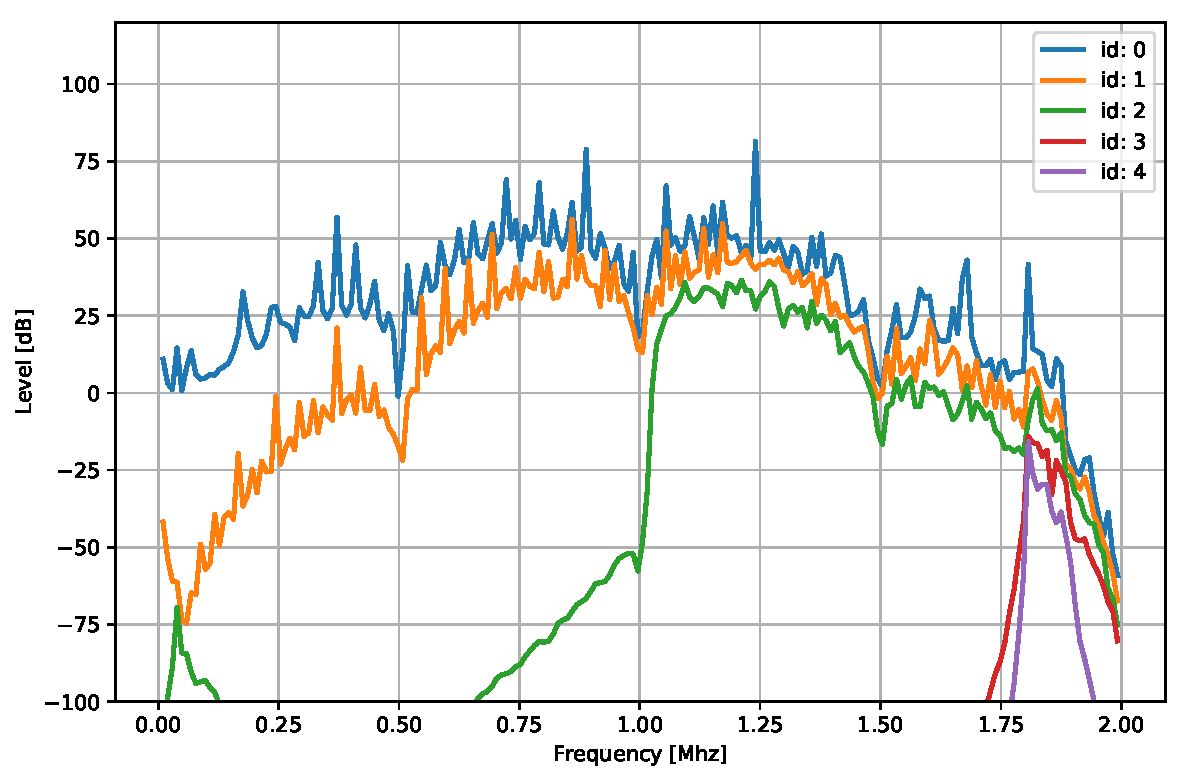
\includegraphics[scale=.5]{images/FreqRes/2DFreqS810Elastic09_SV.pdf}
	\caption{Singular values obtained by the SVD decomposition of the recorded signal from the simulation \ref{FK-Freq-DiagramS8P10M09}}
	\label{SVD-Freq-S8P10M09}
\end{figure} 

Such a study corresponds to the formulation of an eigenvalue problem associated to the elastic operator, defined as finding the pairs $\{(\lambda_k, u_k) \, : \, k \in \mathbb{N} \} \subset \mathbb{R}_+ \times \mathbf{H}^1(\Omega, \Gamma_D)$ solution to the following variational form:

\begin{equation*}
    \label{VariationalEigenProb}
    \mathcal{I}_{\mathbf{C}^{hom}} (u_k, v) = \lambda_k (u_k, v)_{\Omega} \quad \forall v \in \mathbf{H}^1(\Omega, \Gamma_D)
\end{equation*}
where we identify each eigenvalue to the eigenfrequency associated to our problem in the form:
\begin{equation*}
    \lambda_k = \rho^0 (2\pi f_k)^2, \text{ i.e. } f_k = \frac{1}{2\pi} \sqrt{\frac{\lambda_k}{\rho^0}} \quad k \in \mathbb{N}_{*}
\end{equation*}

\begin{rem}
Ket us note in particular that the existence of such pairs is obtained from a classical result of elliptic theory \cite{raviart1983introduction}, \cite{evans2010partial}. Explicitly, it follows since the homogenized coefficients are elliptic and moreover they are bounded which gives us a well-defined bilinear, bicontinuous and coercive operator $\mathcal{I}_{\mathbf{C}^{hom}}(\cdot, \cdot)$ and a linear continuous operator $b(\cdot) := (u_k, \cdot)$ defined respectively on $\mathbf{H}^1(\Omega, \Gamma_D)^2$ and $\mathbf{H}^1(\Omega, \Gamma_D)$.
\end{rem}



It was found numerically a spectrum with abundant eigen-frequencies in bounded intervals of frequency (predicted from the theory), nevertheless the experimental frequency array which was necessary to use for further studies in connection with the real data, showed a neighborhood of at least eigen-frequencies over each experimentally selected frequency. 

In (\ref{EigenValuesComparison}) is shown the frequencies used in the experimental setting used for the simulations in the frequency domain and the eigen-frequencies associated to the operator under study.

\begin{figure}%
    \centering
    \subfloat[Start Bandwidth]{{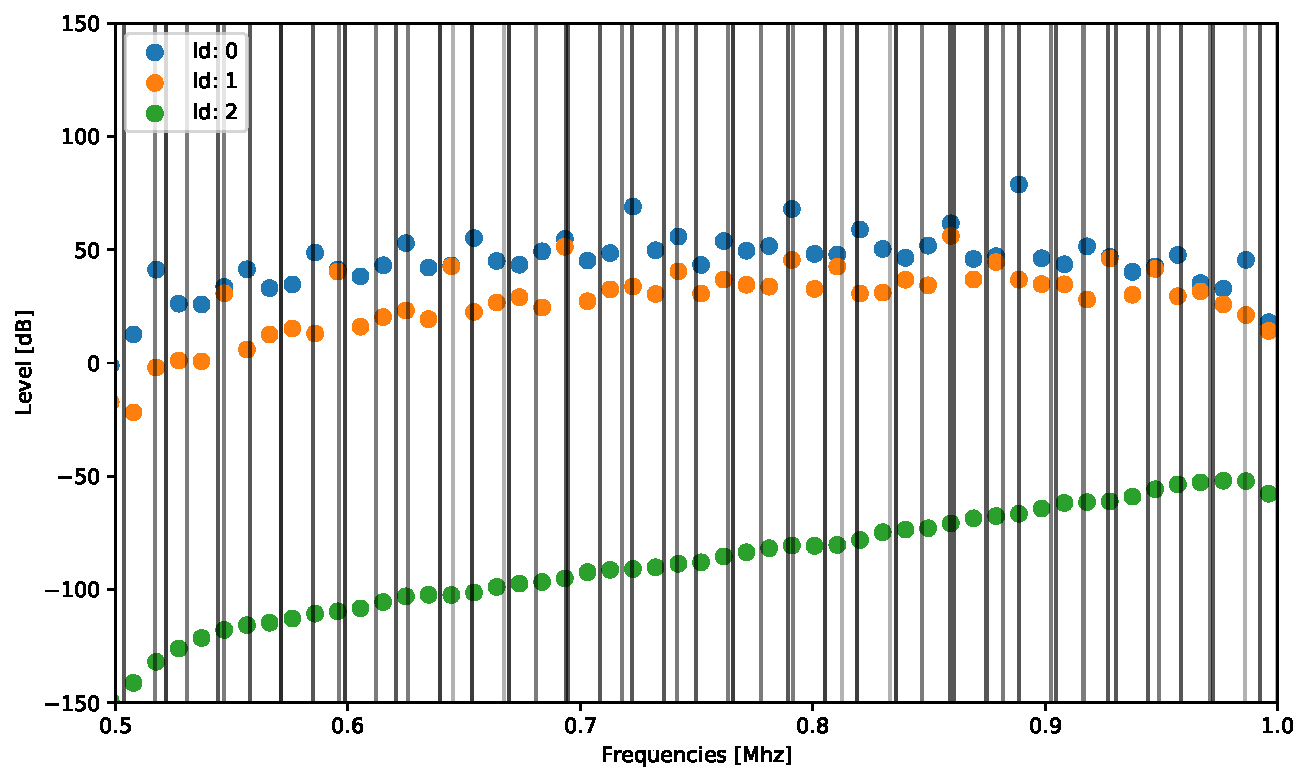
\includegraphics[width=7cm]{images/FreqRes/SingValues-EigenFreqs05-10.pdf} }}%
    \qquad
    \subfloat[End Bandwith]{{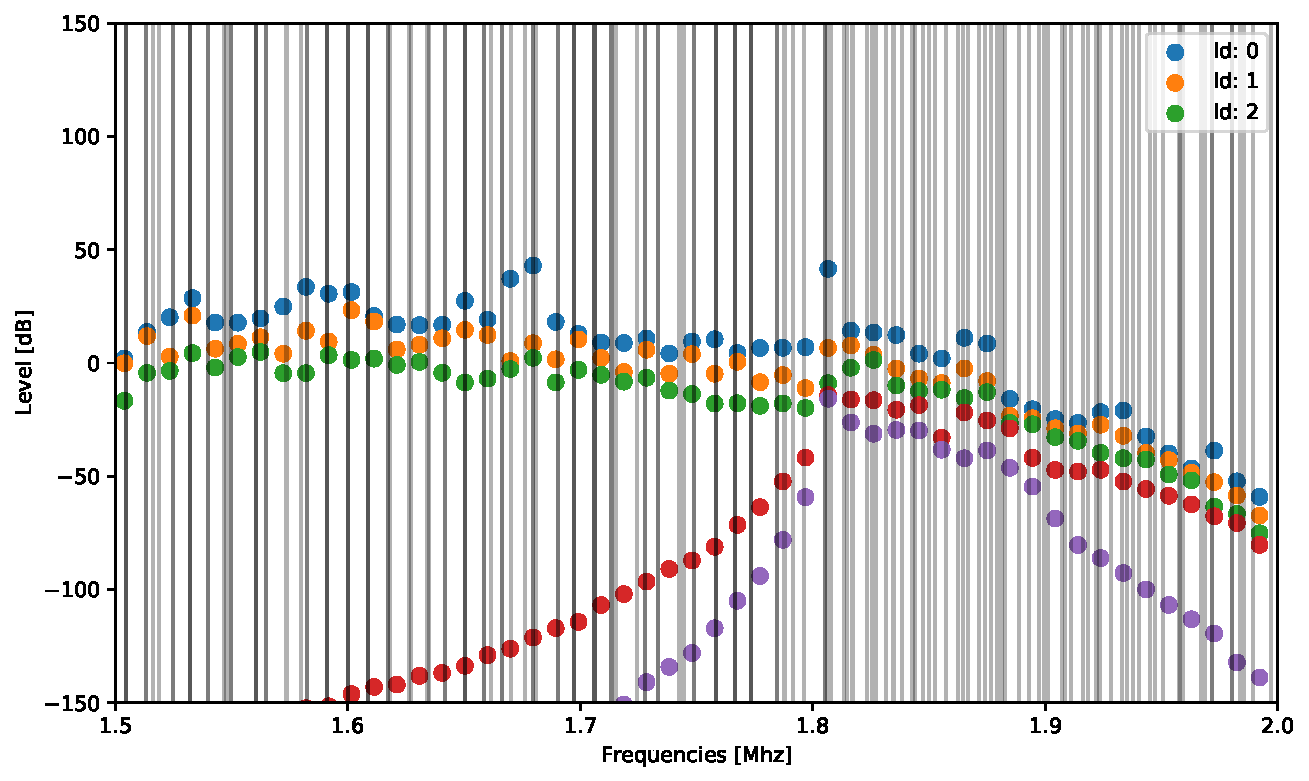
\includegraphics[width=7cm]{images/FreqRes/SingValues-EigenFreqs15-20.pdf} }}%
    \caption{Comparison between Singular Values and Eigen-frequencies: Experimentally its found a increasing sequence of eigenvalues that intersects the experimentally chosen array frequencies.}%
    \label{EigenValuesComparison}%
\end{figure}


\subsubsection{Solution using Attenuation.}
To fix the oscillation observed in the frequency-domain problem we consider adding a $\epsilon$ viscous-like term, such model in particular defines a translation of the eigenfrequencies from the elastic operator to the complex plane thus avoiding the real plane resonances. This implies moreover that we are avoiding the ill-conditioned matrix system from the FEM space discretization.

Fixing a frequency $\omega \in \mathbb{R}$, let us consider solutions in the form: $u(\mathbf{x},t) = e^{2 \pi i \omega t}\hat{u}(\mathbf{x})$, so that $\hat{u}(\mathbf{x})$ solves the equivalent problem in the frequency domain
\begin{equation*}
    \left \{
    \begin{array}{ccc}
        -(2\pi \omega)^2 \rho^0 \hat{u}(\mathbf{x}) - i \epsilon \hat{u}(\mathbf{x}) - \nabla \cdot \sigma(\hat{u}) = \mathbf{0} & \text{ in } \Omega \times [0,T] \\
        \hat{u} = \mathbf{0} & \text{ on } \Gamma_D\\
        \sigma(\hat{u}) \cdot n = \mathbf{F}(\mathbf{x}, \omega) & \text{ on }\Gamma_N \times [0,T]
    \end{array}
    \right .
\end{equation*}
Taking into account that the current \texttt{FEniCS} version doesn't support the usage of a complex coefficient formulation in the variational form, we decompose the solution in its real and complex part as $\hat{u} = \hat{u}_R + i \hat{u}_I$. It follow then the coupled system satisfied for the pair $(\hat{u}_R, \hat{u}_I)$ given by:
\begin{equation*}
    \left \{
    \begin{array}{cc}
        -(2\pi \omega)^2 \rho^0 \hat{u}_R +  \omega \epsilon \hat{u}_I - \nabla \cdot \sigma (\hat{u}_R) = \mathbf{0} & \text{ in }\Omega \times [0,T] \\
        -(2\pi \omega)^2 \rho^0 \hat{u}_I - \omega \epsilon \hat{u}_R - \nabla \cdot \sigma (\hat{u}_I) = \mathbf{0} & \text{ in }\Omega \times [0, T] \\
        \hat{u}_R, \hat{u}_I = \mathbf{0} & \text{ on } \Gamma_D \\
        \sigma(\hat{u}_R)\cdot n, \sigma(\hat{u}_I)\cdot n = \hat{\mathbf{F}}_R, \hat{\mathbf{F}}_I & \text{ on }\Gamma_N
    \end{array}
    \right.
\end{equation*}
which can be solved with the standard tools of \texttt{FEniCS} by the usage of a mixed element for the couple system.

Its shown then on figure \ref{FK-DiagramFreqS8P12M28} the $(f,k)$-diagram associated to the 8-sources simulations setting. It presents natural reflections related to the rectangular 2-dimensional domain used with mixed boundary conditions.
\begin{figure}[!h]
	\centering
	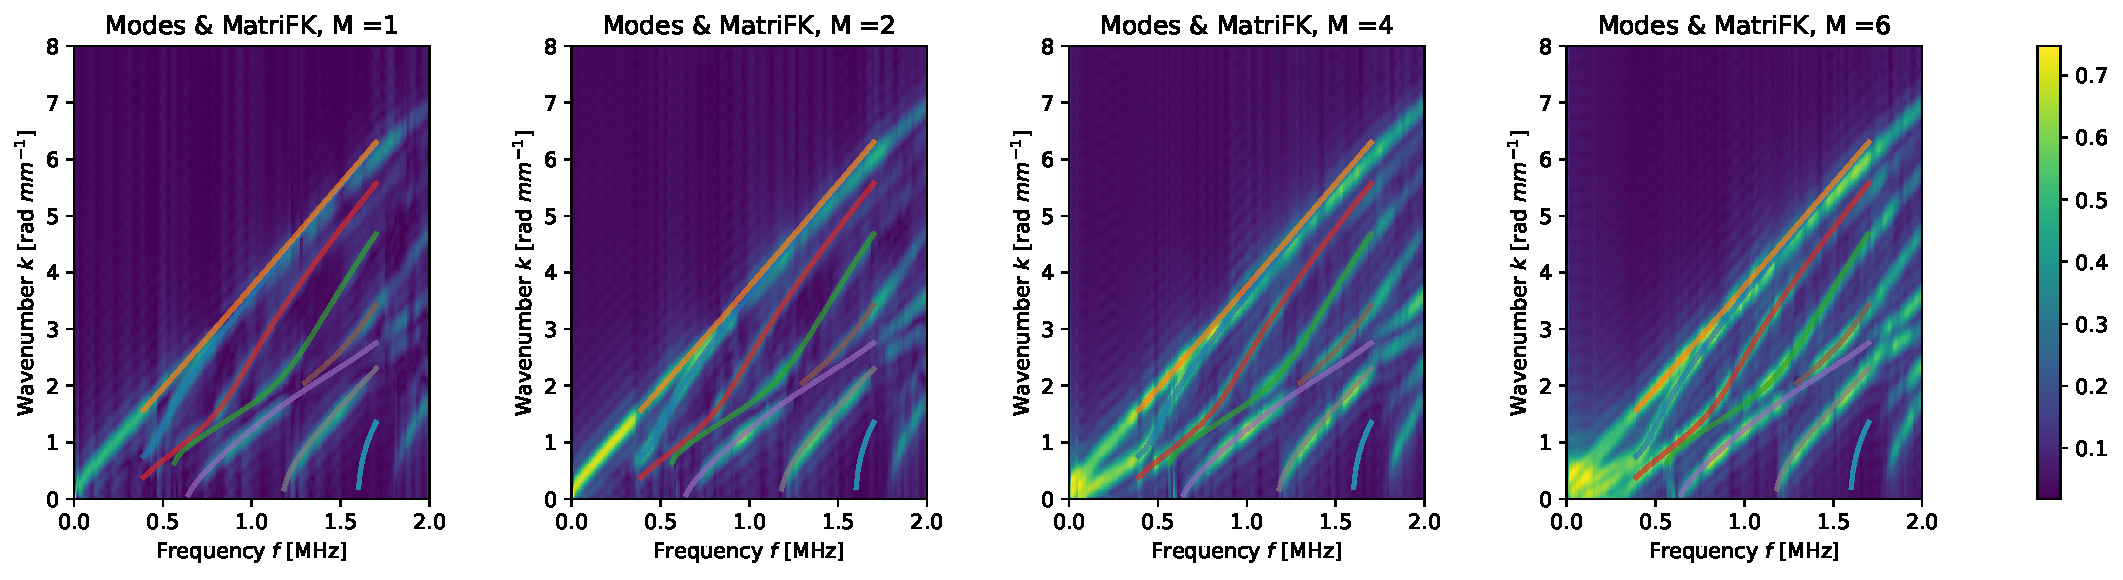
\includegraphics[width=\textwidth]{images/FreqMultSous/2DMixedP12TransIsoFKW28M400_y.pdf}
	\caption{Numerically Simulated $(f,k)$-diagram of 2D Transverse Elastodynamic Model: Setting of 1 source with $3\%$ porosity and thickness of $3.0 [mm]$.}
	\label{FK-DiagramFreqS8P12M28}
\end{figure}

Nevertheless, from the figure \ref{SVD-S1P7M30} of main modes $[dB]$ associated to the recorded signal, its observed vanishing oscillation of the modes, thus numerically avoiding the eigenfrequencies, the main resonance cause.
\begin{figure}[!h]
	\centering
	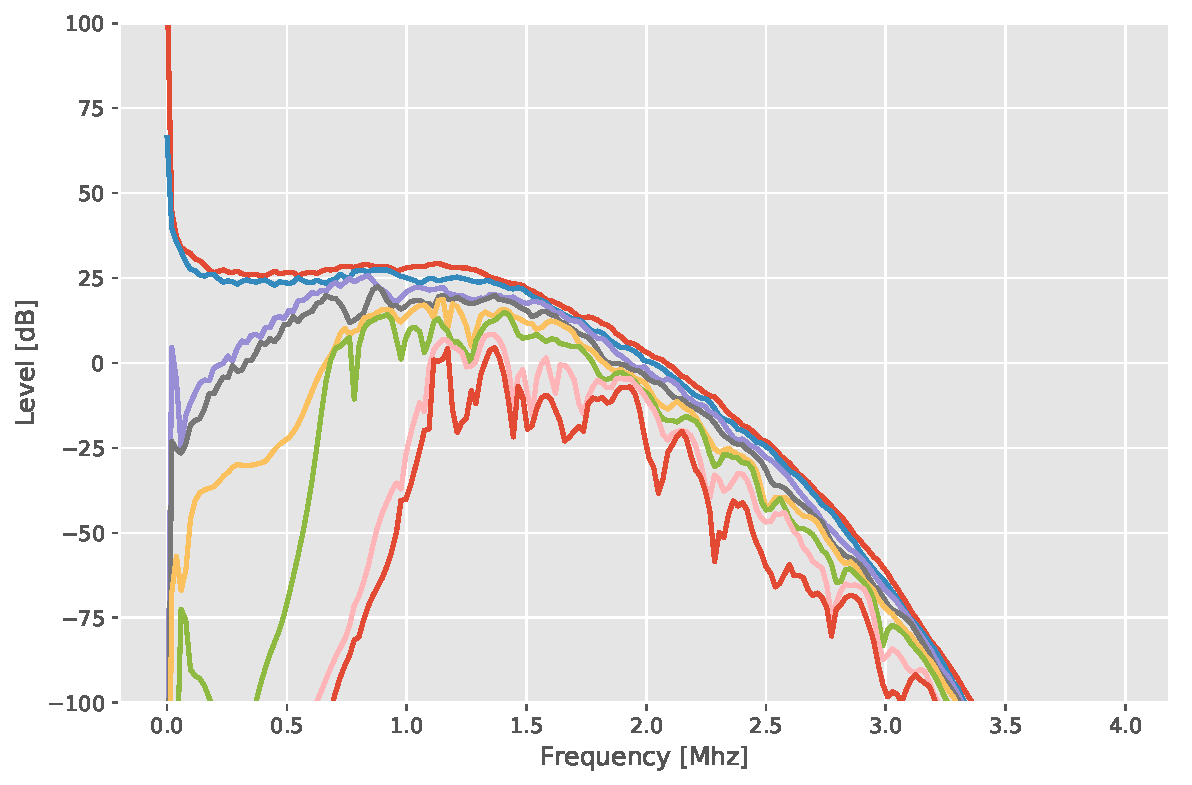
\includegraphics[scale=.5]{images/FreqMultSous/2D-FreqSimP12W28eKV_SV.pdf}
	\caption{Singular values obtained by the SVD decomposition of the recorded signal from the simulation \ref{FK-DiagramFreqS8P12M28}}
	\label{SVD-FreqS8P12M28}
\end{figure}


\subsection{Simulation of Wave Propagation on 3-dimension}
Following the 2-dimensional case, its now studied the effect of radial wave behavior on the recorded signal, validating in particular the experimentally obtained results that neglect the non-axial wave-guide propagation. 
Such procedures imply the creation of adaptive meshes to the complex cortical bone geometry, where open-source software such as \texttt{iso2mesh}, \texttt{CGAL} is used for its generation and in particular a created a pipeline of mesh generation from $\mu$-CT images.

\subsubsection{Half-Cylinder Case}
A half-cylinder mesh is proposed as first approximation to the 3-dimensional real cortical bone sample from the $\mu$-CT images. In this case, avoiding the non-uniformity characteristic of the bone surface, its tested the waveguide propagation and distortion generated by the natural curvature of the mesh.


\subsubsection{Rugous Exterior}
The mesh generation is done, using the following pipeline dataflow:

\begin{figure}[!h]
	\centering
	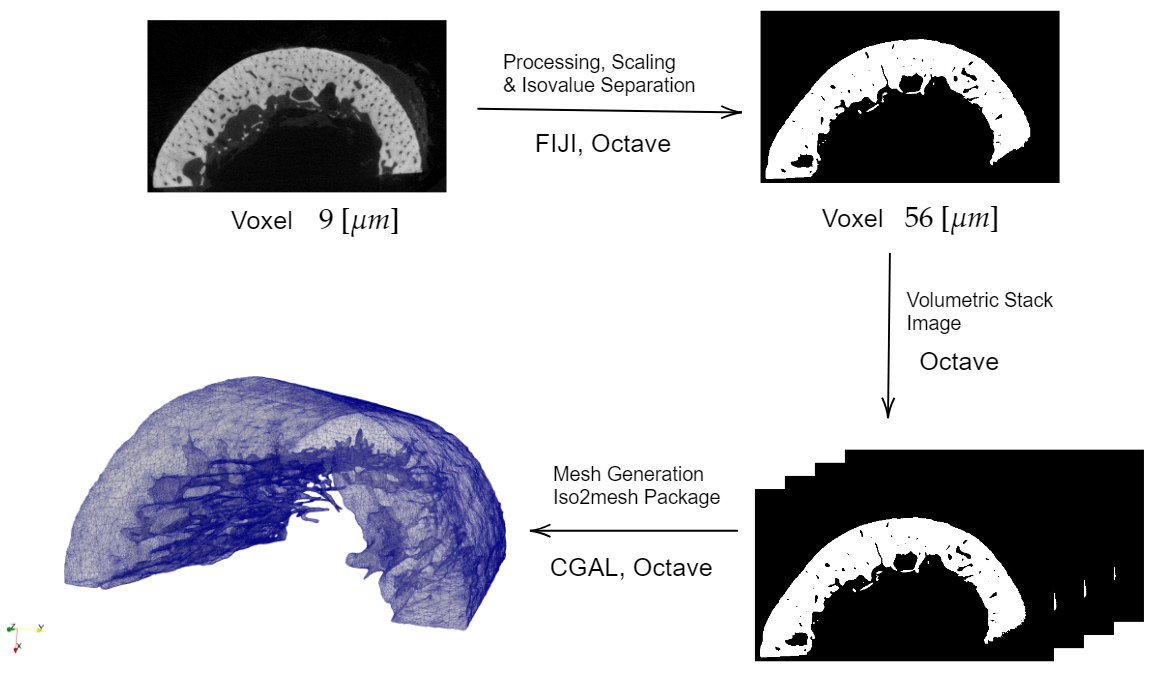
\includegraphics[scale=.5]{images/ImgExt/DiagramMeshGeneration.png}
	\caption{Pipeline: The mesh generation involves a sequence of different softwares that generates the desired domain where the simulations takes place.}
	\label{DiagramMeshGeneration}
\end{figure} 

\subsubsection{Fully Porous Material}
The save Pipeline (\ref{DiagramMeshGeneration}) is used for the mesh generation, now without homogenized coefficients and therefore taking into account the variation on the elastic coefficients depending on the presence of mesoscale structure and cavities.
